% !TEX encoding = UTF-8 Unicode
%!TEX root = memoria.tex
% !TEX spellcheck = es-ES
%%=========================================
\chapter{Estado del arte}
%%=========================================

\section{Neuroimagen}

Las técnicas de neuroimagen han cambiado el panorama en que los científicos abordan las hipótesis sobre la anatomía funcional del cerebro, especialmente en relación con el comportamiento y los desordenes clínicos. \cite{bold_fmri}

\subsection{Anatomía básica del cerebro}

El cerebro humano está compuesto por alrededor de $10^{11}$ \hyperref[eda:neurona]{neuronas} y sobre $10^{4}$ sinapsis por cada neurona comprimidas en un volumen de unos $1,400cm^{3}$.

\begin{figure}[H]
  \centering
    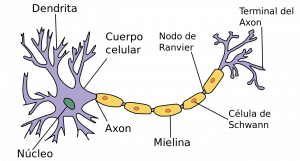
\includegraphics[scale=0.75]{img/neurona.png}
  \caption{Neurona cerebral}\label{eda:neurona}
\end{figure}


Las neuronas están densamente conectadas y tienen muchas \hyperref[eda:neurona]{dentritas}. Asi mismo los axones conducen las señales electricas y están recubiertos por mielina. La mielina es un factor determinante a la hora de establecer la señal y el contraste de la resonancia magnética. Las neuronas se organizan en tres tipos de \hyperref[eda:tejidos]{tejidos}:

\begin{itemize}
	\item Sustancia Gris (GM): Contiene numerosos cuerpos celulares (somas) y relativamente pocos axones cubiertos de mielina. Se asocia con la función del procesamiento de la información, es decir con la capacidad del razonamiento. Se localiza en la superficie del cerebro, formando la corteza cerebral, que corresponde con la organización mas compleja de todo el sistema nervioso.
	\item Sustancia Blanca (WM): Principalmente estáformado por un gran número de axones(parte de la neurona encargada de transmitir l información) cubiertos de mielina y contiene relativamente pocos cuerpos celulares. Se corresponde con la parte interior del cerebro.
	\item Fluido Cerebroespinal (CSF): Para la protección mecánica básica e inmunológica del cerebro.
\end{itemize} 

\begin{figure}[H]
  \centering
    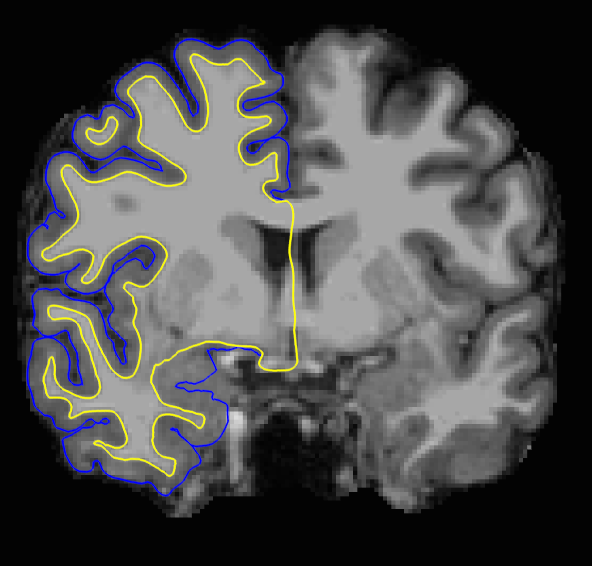
\includegraphics[scale=0.60]{img/tejidos.png}\label{eda:tejidos}
  \caption{El cerebro requiere el 20\% de la energía total del cuerpo y entre el 60 y 80\% de esta energía es utilizada en las conexiones cerebrales (comunicación entre neuronas)}
\end{figure}

\cite{brainhack}

\section{Datos del cerebro}

El campo de la neuroimagen incluye el uso directo o indirecto de varias técnicas de imagen estructural o funcional del cerebro.

Los datos anatómicos o \hyperref[eda:anat]{imagen} anatómica describen el tamaño, la forma y la integridad de las estructuras de los tejidos en el cerebro. Se obtiene al realizar una resonancia magnética convencional y nos permite visualizar de manera contrastada la sustancia gris y la sustancia blanca.

\begin{figure}[H]
  \centering
    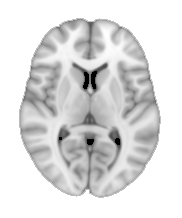
\includegraphics[scale=0.75]{img/anat.png}
  \caption{Imagen estructural del cerebro}\label{eda:anat}
\end{figure}

Los datos \hyperref[eda:func]{funcionales} calculan los patrones de activación de las diferentes poblaciones de neuronas o regiones dentro del cerebro. Permite detectar zonas de mayor oxigenación en el cerebro cuando el paciente está realizando una actividad o en estado de reposo.

\begin{figure}[H]
  \centering
    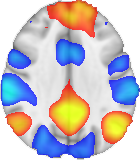
\includegraphics[scale=0.75]{img/func.png}
  \caption{Imagen funcional del cerebro}\label{eda:func}
\end{figure}
\cite{brainhack,fmri_oxford}

\subsubsection{Datos funcionales}

Mide la actividad neuronal a través de la señal dependiente del nivel de oxigenación de la sangre de cada voxel (\hyperref[glos:bold]{BOLD}). La actividad neuronal causa una mayor demanda de energía, a través de un proceso llamado respuesta hemodinámica la sangre libera oxigeno a las neuronas activas, disparadas a una tasa mucho mayor en comparación con las neuronas inactivas. \cite{brainhack,bold_fmri}

\begin{figure}[H]
  \centering
    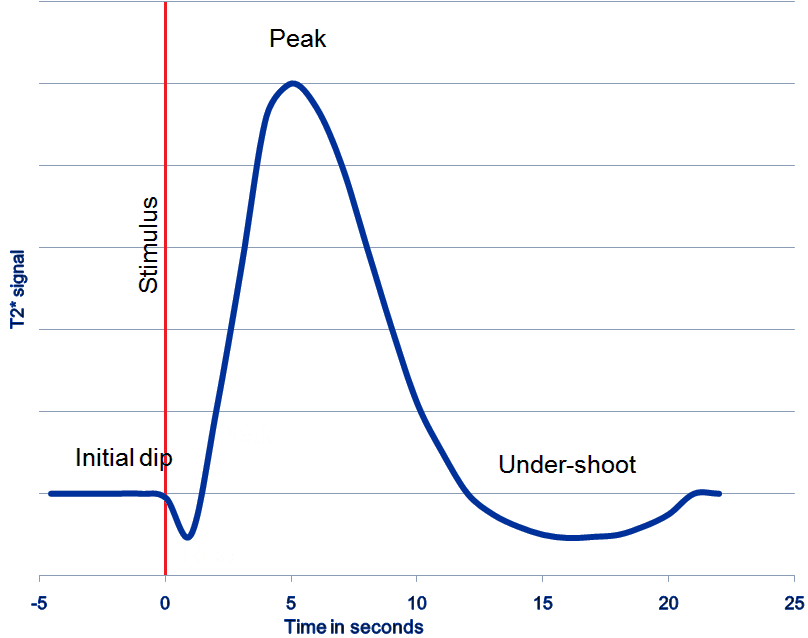
\includegraphics[scale=0.5]{img/bold.png}
  \caption{Respuesta hemodinámica}
  \label{eda:bold}
\end{figure}

Mientras que la actividad neuronal ocurre en milisegundos, la respuesta hemodinámica es más lenta y toma alrededor de 5 segundos enn alcanzar su máximo como se puede ver en la figura \ref{eda:bold} seguido por un descense inferior al nivel basal aproximadamente a los 15 segundos.

En la mayoría de las aplicaciones la resolución espacial se encuentra entre 1 y 5mm. La resolución temporal suele estar entre 0.5 y 3 segundos ~\ref{eda:resol}.\cite{courserafmri1,brainhack,fmri_oxford}

\begin{figure}[H]
  \centering
    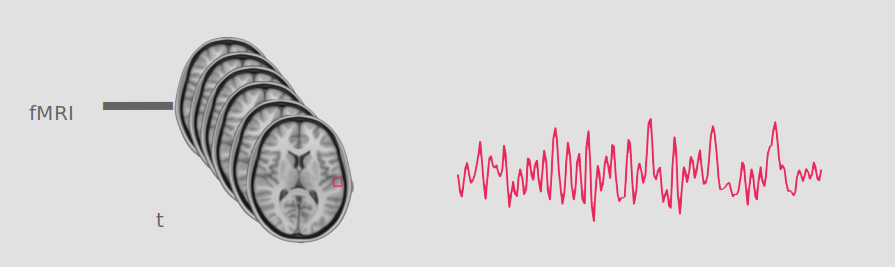
\includegraphics[scale=0.5]{img/resol.png}
  \caption{Resolución temporal}
  \label{eda:resol}
\end{figure}

Existen dos modalidades principales de fMRI:

\begin{itemize}
	\item \textbf{Task fMRI}: El sujeto realiza una tarea durante el escaner
	\item \textbf{Rest fMRI}: El sujeto se encuentra relajado y no hace ni piensa en nada durante el escaner.
\end{itemize}

El presente experimento se obtiene un conjunto de datos basado en la segunda modalidad.

\section{Estandar de imágen médica: DICOM}

Del Inglés \textit{Digital Imaging and Communications in Medicine} fué creado por \textit{National Electrical Manufacturers and Association} para permitir la visualización y distribución de imágenes médicas. Es el estandar mundialmente reconocido para este fin.

DICOM tiene un conjunto muy amplio de servicios, la mayoría de los cuales implica transmisión de datos sobre la red, y el formato de fichero en que se sustenta es en realidad una ampliación posterior y de menor importancia del estándar. Queda recogido en el PS3.10 \cite{dicom} del estandar.\cite{nema}

Un único archivo DICOM contiene la cabecera, la cual contiene información sobre el nombre del paciente, el tipo de escaner, la dimensión de la imágen y otros metadatos, además de todos los datos de la imágen en formato binario. Es posible comprimirlo a fin de reducir el tamaño de la imágen. A menudo son separados en \textit{slices} de dos dimensiones, pero pueden ser combinadas en un único archivo.


\subsection{Cabecera DICOM}

La siguiente \hyperref[dicom:dummy_image]{imagen} muestra un hipotético archivo DICOM. En este ejemplo, los primeros $794$ bytes son usados para la cabecera DICOM, la cual informa de la dimensión de la imágen y guarda otra información sobre el escaner. El tamaño de la cabecera puede variar en función de cuanta informaión se almacena en ella. En este caso se encuentra una imagen de $109x91x2$ voxels, con una resolución de un byte por voxel (por tanto el tamaño total de la imagen es de 19838 bytes). La imagen se encuentra a continuación de los datos de la cabecera, generalmente en el mismo archivo.

\begin{figure}[H]
  \centering
    \label{dicom:dummy_image}
    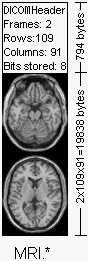
\includegraphics[scale=0.75]{img/dcmi.png}
  \caption{Imagen estandar  DICOM}
\end{figure}

El estandar de almacenamiento que recoge DICOM, reserva los 128 primeros bytes para el preambulo(el cual generalmente no contiene información, son todo ceros) segido por los caracteres `D', `I', `C' y `M'. Tras estos caracteres aparece la información de la cabecera, la cual se organiza en ``grupos''. Por ejemplo el grupo \textit{002hex} en la siguiente \hyperref[dicom:dummy_header]{imagen} es el grupo de los metadatos del archivo, en el siguiente ejemplo contiene tres elementos: uno define la longitud del grupo, otro guarda la versión del archivo y el tercero almacena la sintaxis de transferencia.

\begin{figure}[H]
  \centering
    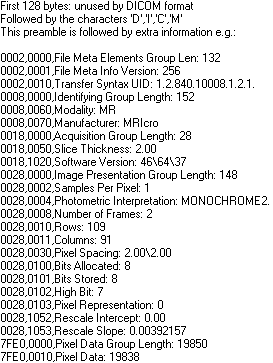
\includegraphics[scale=0.75]{img/header.png}
  \caption{Cabecera  DICOM}\label{dicom:dummy_header}
\end{figure}

Los elementos requeridos dependen del tipo de imagen, en la parte 3 del archivo DICOM de ejemplo en la imagen \ref{dicom:dummy_header} aparece como `MR' (0008:0060), por tanto tendrá que contener los elementos que describen un \textbf{MRI}. La ausencia de este elemento supone una violación del estandar.

Un elemento de particular importancia es \textbf{002:0010} (ver la tabla \ref{dicom:tab_sintaxis}), el cual define el identificador único de transferencia de sintaxis \textbf{Transfer Syntax Unique Identification}. Este valor informa la estructura de los datos de la imagen, revelando si los datos han sido comprimidos o no (lo que podría suponer perdidas en los datos de altas frecuencias).

\begin{table}[H]
  \centering
    	\tiny
  \begin{tabular}{|c|l|}
    % body of tabular environment 
    \hline
    Transfer Syntax UID	& Definition \\
    \hline
    1.2.840.10008.1.2.x	& Raw data, Eplicit VR x = 1: Little Endian x = 2: Big Endian \\
	1.2.840.10008.1.2.4.xx &	JPEG compression xx = 50-64: Lossy JPEG xx = 65-70:Lossless JPEG \\
	1.2.840.10008.1.2.5	& Lossless Run Length Encoding  \\
    1.2.840.10008.1.2 		&	Raw data, Implicit VR, Little Endian \\	
    1.2.840.10008.1.2.4.xx & JPEG compression xx = 50-64: Lossy JPEG xx = 65-70: Lossless JPEG \\
    1.2.840.10008.1.2.5 & Lossless Run Length Encoding \\
    \hline
  \end{tabular}
  \caption{Definición de transferencia de sintáxis}\label{dicom:tab_sintaxis}

\end{table}

Además de informar sobre la técnica de compresión (si existe), el \textbf{UID} de la sintaxis de transferencia infroma del orden de los bytes de datos sin procesar. Cada host puede almacenar de forma diferente los valores \textbf{integer} (big endian y little endian ordering). Si consideramos un entero de 16 bits con el valor 257: el byte más significativo almacena el valor 01 (= 255), mientras que el byte menos significativo almacena el valor 02. Algunas computadoras guardarán este valor como 01:02, mientras que otras lo almacenarán Como 02:01. Por lo tanto, para los datos con más de 8 bits por muestra, un visor DICOM puede necesitar cambiar el orden de bytes de los datos para que coincida con el orden utilizado por el equipo.

\section{Estandar de imágen médica: NIFTI}

\subsection{Cabecera}

Hereda su estructura de 348 bytes del formato estandar \textbf{ANALYZE}. En los últimos cuatro bytes de la cabecera se corresponden con el campo ``mágico'' que indica si la cabecera y la imagen están en un único archivo ($magic = n+1|0$) o en dos separados ($magic = ni1|0$). Añade cuatro bytes adicionales al formato \textbf{ANALYZE} indicando la \textit{extensión} de la cabecera. Por defecto esos cuatro bytes son ceros.

%%=========================================
\section{Neuroimagen de temblor esencial}

El temblor esencial (\hyperref[glos:et]{ET}) es uno de los desordenes neurológicos más comunes con una prevalencia del 0.9\% en la pblación general, que incrementa con la edad, con una estimación de aproximadamente 5\% sobre los individuos de 65 años. El comienzo clinico es bimodal, algunos de los sintomas se presentan en una fase muy temprana de la vida, mientras otros sintomas se presentan en una fase más tardía. \cite{movedisorder,ethandbook}

Algunos estudios recientes sugieren que se trata de un proceso de evolución lenta degenerativa con sintomas que no están relacionados con el sistema motor como disfunciones cognitivas, ansiedad, depresión y perdida de audición.
El diagnóstico clínico suele realizarse basado en el historial médico y los resultados de un examen neurológico. \cite{movedisorder}

\subsection{Fisiopatología}

La fisiopatología del ET solo se entiende parcialmente, pero algunos estudios clínicos y de imagen apuntan a que el cerebelo está involucrado.Algunos estudios neurológicos y de animales,post-mortem, indican que la oliva inferior, el cerebelo, el núcleo rojo, el tálamo y el cortex y sus neurotransmisores están involucrados. Estas areas conforman la red conocida como \hyperref[te:cerebelo-talamo-cortex]{cerebelo-tálamo-corticales} (CTC).\cite{rolectc,neuessentialsinet}

\begin{figure}[H]
  \centering
    \label{et:cerebelo-talamo-cortex}
    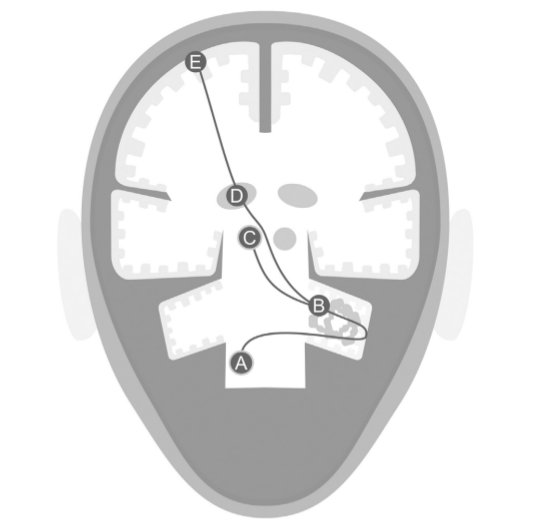
\includegraphics[scale=0.5]{img/cerebelo-talamo-cortex.png}
  \caption{Red del temblor: A)Oliva inferior; B) Núcleo dentado; C)Núcleo rojo; D)Tálamo; E) Cortex-motor} Imágen extraida de \cite{neuessentialsinet}
\end{figure}

Los estudios individuales basados en imágen estructural no han revelado anomalías significativas en pacientes con temblor esencial. Si embargo, estudios patólogicos más avanzados han mostrado cambios estructurales \cite{neuessentialsinet}.
Los estudios de imagen funcional son capaces de asociar el temblor esencial con la actividad cerebral en reposo o mientras realiza una actividad. Las diferencias en los mapas de activación podrían indicar oscilaciones primarias en las areas de los circuitos con perdidas o en las regiones compensatorias. También podrían ser causadas por la inhibición o excitación de cambios neurodegenerativos \cite{neuessentialsinet}.
 

%%=========================================
\section{Preprocesado de neuroimágen}
\subsection{Neuroimagen funcional fmri}
\subsection{Neuroimagen anatómica MPRAGE}
%%=========================================
\section{Mapa cerebral}
%%%=========================================
\section{Análisis no lineal}
%%%=========================================
\subsection{Teoría de la información}
Existen estudios basados en la teoría de la información como el estudio del incremento de la entropía con la edad en la imagen funcional que recoge \cite{Yao2013}.
\subsubsection{Entropía espectral de Shannon}
\subsubsection{Entropía de permutación}